\hyphenation{se-para-tion}
\hyphenation{theo-re-ti-cal}
\hyphenation{handed-ness}
\hyphenation{fo-llo-wing}
\hyphenation{ac-cor-ding}

%______________________ Theory ______________________
\chapter{The LHC Accelerator and the CMS Experiment}\label{ch:lhcandcms}
In the 1960s Peter Higgs and others {\color{red}\ital{need ref}} put up the finishing touches on a theory combining three of the four fundamental forces. This theory became to be known as the Standard Model (SM) of particles physics. It predicted the existence of several particles which were discovered in the following decades. However, one particle was proving to be elusive, the so-called Higgs bosson. With this in mind the European Organization for Nuclear Research (CERN) started plans to build an accelerator large enough to be able to find this elusive particle. Hence, the Large Hadron Collider (LHC) was born. 

\section{The LHC Accelerator}
A circular ring of 27 Km in circumference, the LHC was built at the French-Swiss border outside Geneva, Switzerland, see figure \ref{fig:cern}. 

\begin{figure}[!h]
  \centering
  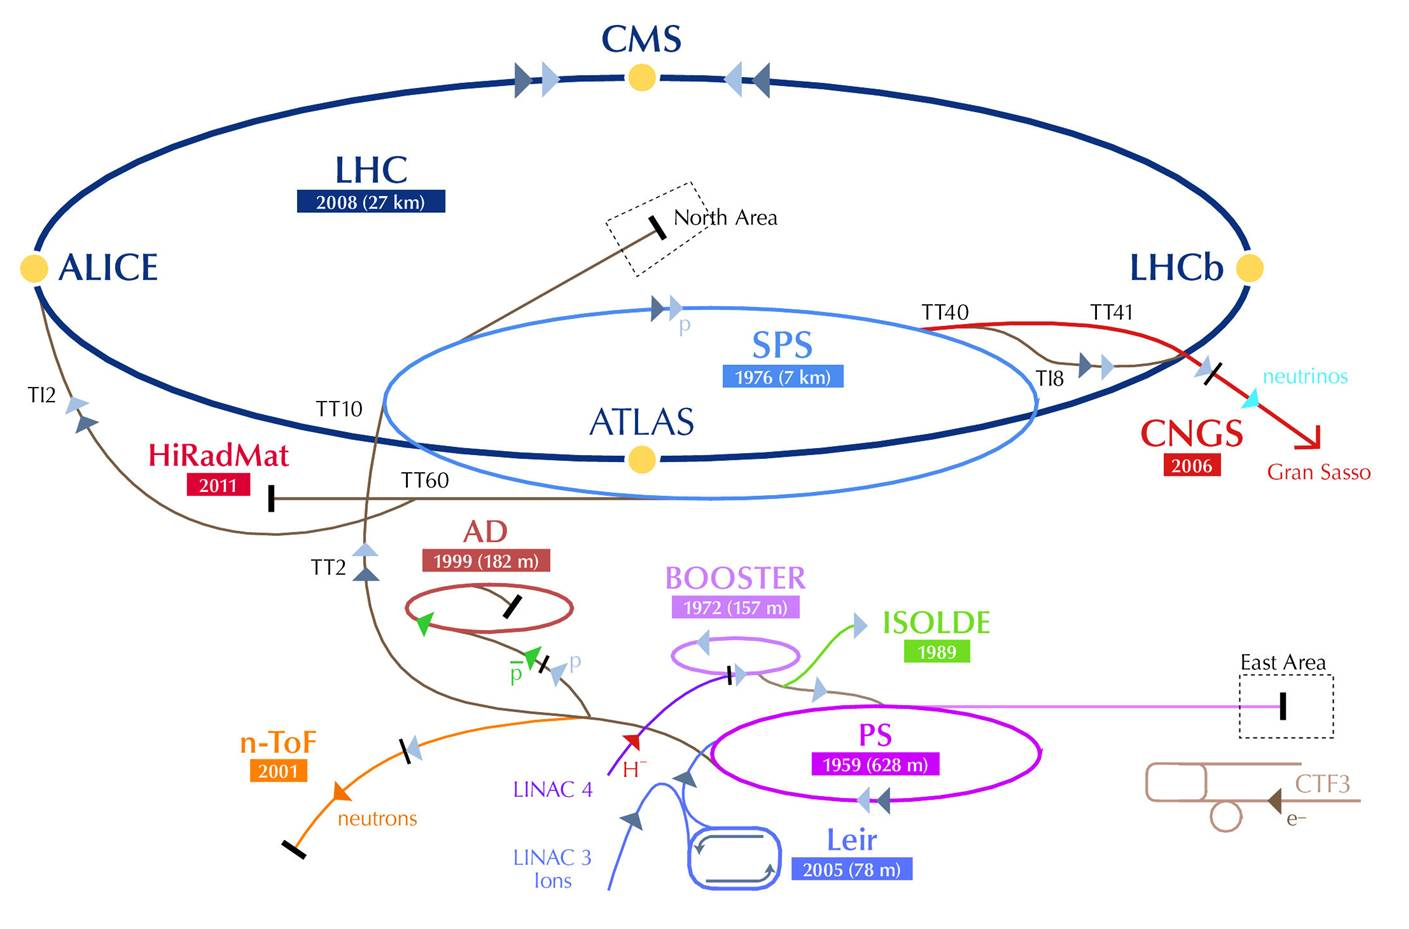
\includegraphics[width=0.7\textwidth]{../images/ch2/cern_complex}
  \caption[The CERN acceleration \ital{facilities}]{The CERN acceleration \ital{facilities} showing the location of the four main experiment as well as the acceleration process[need ref].}\label{fig:cern}
\end{figure}




Four experiments were designed and build to test different physics theories and search for undiscovered particles at the LHC. Two of them, A Toroidal Large Aparatus (ATLAS)\cite{atlas} and the Compact Muon Solenoid (CMS)\cite{cms_doc} are large multipurpose experiments. The third experiment is LHCb \cite{lhcb}, which is specifically dedicated to study B-meson physics, the last experiment ALICE \cite{alice}, A Large Ion Collider Experiment, was design to investigate heavy ion collisions.



%\subsection{LHCb}
%\subsection{Atlas}
%\subsection{ALICE}
\section{CMS}

\begin{figure}[!h]
  \centering
  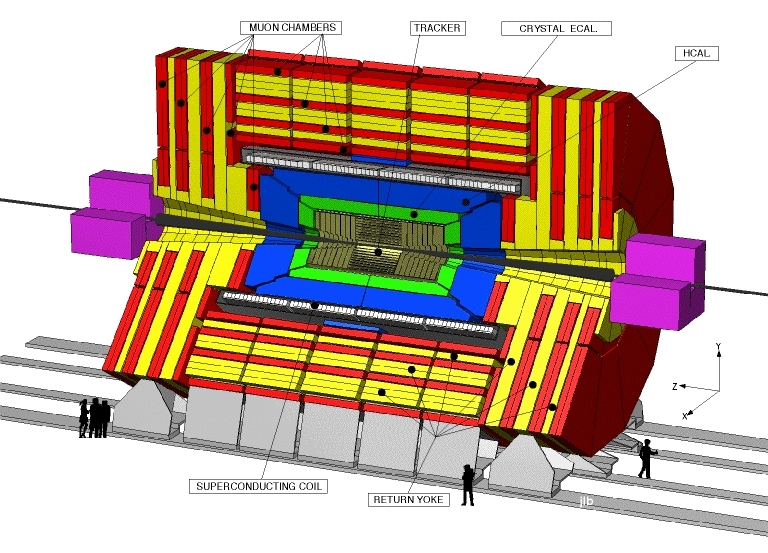
\includegraphics[width=0.7\textwidth]{../images/ch2/cms_layout}
  \caption[CMS cross sectional view]{CMS cross sectional view.}\label{fig:cms_layout}
\end{figure}

\begin{figure}[!h]
  \centering
  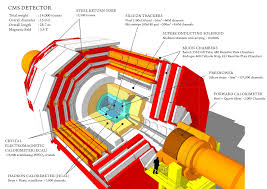
\includegraphics[width=0.7\textwidth]{../images/ch2/cms2}
  \caption[CMS cross sectional view]{CMS cross sectional view.}\label{fig:cms_layout}
\end{figure}


\begin{figure}[!h]
  \centering
  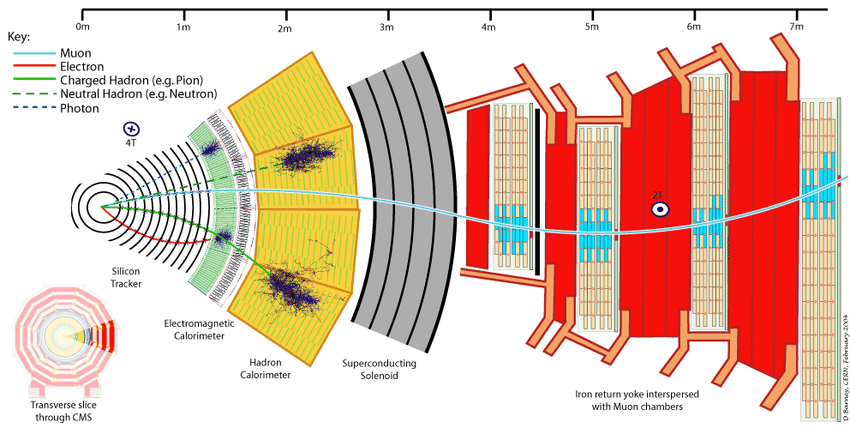
\includegraphics[width=0.7\textwidth]{../images/ch2/cms_cross}
  \caption[CMS cross sectional view]{CMS cross sectional view.}\label{fig:cms_cross}
\end{figure}
\subsection{The Tracker Detector}
\subsection{The Electromagnetic Calorimeter}
\subsection{The Hadronic Calorimeter}
\subsection{The Muon Chambers}

%______________________ INTRODUCCION ______________________
%\section{Introduction}
%\label{secc:Intro_th}



